\documentclass[class=scrbook, crop=false]{standalone}
\usepackage[subpreambles=true]{standalone}
\ifstandalone
    % WARNING: Proceed with caution!

% -----------------------------------------------------------------------------------
% For package standalone
% -----------------------------------------------------------------------------------
\usepackage{import}

% -----------------------------------------------------------------------------------
% Language and typeset
% -----------------------------------------------------------------------------------
\usepackage[ngerman, english]{babel}

\usepackage{subcaption}
% Umlauts and other special characters (UTF-8)
% \usepackage[utf8]{inputenc}
\usepackage{fontspec}
\setsansfont{Arial}
% \usepackage[T1]{fontenc}  % Enable accented characters and umlauts
% LuaLatex doesn't need fontenc and uses UTF-8
% \usepackage{lmodern}  % Font face


% --------------------------------------------------------------------------------
% Page formatting
% --------------------------------------------------------------------------------
% Change the header/footer for chapter beginnings and normal pages
\usepackage[automark,headsepline]{scrlayer-scrpage}

% The package provides an easy and flexible user interface to customize the page
% layout, implementing auto-centering and auto-balancing mechanisms
% WARNING: WHEN CHANGING BCOR (Binding correction), the cover needs reworking!...
\newcommand{\theBCOR}{15mm}  % Define binding correction
\usepackage[
    bindingoffset=\theBCOR,
    % showframe, % Show boxes which indicate margins and paddings
    bottom = 3.5cm, % Margins
      left = 2.5cm,
     right = 2.5cm
] {geometry}

% The package 'float' provides a container for document objects which can not be
% broken over pages, such as tables and figures
% Needed for table and figure indexes  
\usepackage{float}

% support for landscape layout
\usepackage{lscape}

% support of \tablenotes command to add notes under table
\usepackage{threeparttable}

% To allow drawing more professional tables
\usepackage{booktabs}

% --------------------------------------------------------------------------------
% Contents
% --------------------------------------------------------------------------------
% Vector graphics (for Cover page)
\usepackage{tikz} 

% Allows additional parameters when including images
\usepackage{graphicx}

% Roman font family for all headings
\addtokomafont{disposition}{\rmfamily}

% Set the line spacing to 1.5
\usepackage[onehalfspacing]{setspace}

% Improves overall text spacing
% http://www.khirevich.com/latex/microtype/
\usepackage[stretch=10]{microtype}

% Math symbols like mu outside the math environment
\usepackage{textcomp}

% A comprehensive (SI) units package∗
% For defining SI units
\usepackage[
    range-units=single,         % Formatting ranges with single unit indication: 1 - 2 m
    range-phrase=-,             % Phrase for range: 1 - 2 m vs 1 to 2 m
    separate-uncertainty=true,  % sets +- between value and uncertainty 
    multi-part-units=repeat     % In expressions with multiple values (multi part numbers) 
                                % the unit is printed each time: 1 mm x 1 mm
] {siunitx}
% https://tex.stackexchange.com/questions/124488/multi-part-numbers-and-units-in-siunitx

% Allows Sourcecodes with highlighting 
\usepackage{listings}

% This package provides user control over the layout of the three basic list
% environments: enumerate, itemize and description
\usepackage{enumitem}
\setlist{nosep} % Remove the vertical space between \item elements in all lists

% ToDo Notes
% \setlength{\marginparwidth}{2cm}
\usepackage{todonotes}
\setuptodonotes{inline, inlinepar}
\reversemarginpar  % Put ToDo notes on the binding's side
% \usepackage{soul} % Colorful ToDo notes

% Check out colors here http://latexcolor.com/
\usepackage{xcolor}

\usepackage{amsmath}    % alignment of equations

% --------------------------------------------------------------------------------
% Other elements
% --------------------------------------------------------------------------------
% Blindtext: Organic looking text dummy
\usepackage{blindtext}

% Hyperlinks within the document (PDF)
% "hidelinks" hides visual highlighting of links
\usepackage[hidelinks]{hyperref}

% Package for Glossary and Index (Acronyms are listed in a separate list) 
\usepackage[acronym, nogroupskip]{glossaries}[=v4.49] % groupskip: alphabetic grouping of entries

\usepackage{xltabular}   % <------- FOR glossaries

% Integration and management of bibliographies
\usepackage{csquotes}   % backend=biber in biblatex needs this package
\usepackage[
    style=ieee,   % style of the bibliography, entries are sorted in alphabetic order. "ieee" is another common style.
    backend=biber,      % based on package 'biber' 
    bibencoding=ascii   % ASCII Text encoding; may use "utf8" instead
] {biblatex}

% --------------------------------------------------------------------------------
%                               PATHS & FILES
% --------------------------------------------------------------------------------
% Fix paths for standalone compiling
\ifstandalone
    \def \home {..}
\else
    \def \home {.}
\fi

% Package: scrlayer-scrpage
% \def \stylePath {\home/settings+/style/page}
\input{\home/settings+/style/page}  % Load page style

% Package: graphicx
\graphicspath{{\home/images/}}  % Set path to images

% Package: listings
\input{\home/settings+/style/code.tex}  % Set path to style file
\lstset{inputpath={\home/code/}} % Default path to code listings

% Package: glossaries
\input{\home/settings+/style/symbols}  % Set path to symbols list style file
\input{\home/settings+/style/acronyms}  % Set path to acronym list style file
% -------------------------------------------------------------------------------
%               Listing of all Glossary and Acronym Entries 
%                           use as shown below
% -------------------------------------------------------------------------------

% ==== EXEMPLARY ENTRY FOR SYMBOLS LIST =========================================

% ==== EXEMPLARY ENTRY FOR ACRONYMS LIST ========================================
% \newacronym{#label}{#acronym}{#long_form}

% define new command for custom arconym entry with only two arguments
% fabricates an easier way to use \newacronym 
\newcommand{\acroX}[2]{\newacronym{#1}{#1}{#2}}
% \acroX{label and arconym}{long name}
% \acroX{CD}               {Compact Disk}

\newcommand{\acroY}[3]{\newacronym{#1}{#2}{#3}}
% \arcoY{label}{acronym}{long name}
% \acroY{CD}   {cd}     {Compact Disk}
 
\newacronym{AEP}{AEP}{Imbalance price}
\newacronym{aFRR}{aFRR}{Automatic Frequency Restoration Reserve}


\newacronym{reBAP}{reBAP}{Uniform imbalance price}
\newacronym{TSO}{TSO}{Transmission System Operator}
\newacronym{FCR}{FCR}{Frequency Containment Reserve}
\newacronym{mFRR}{mFRR}{Manual Frequency Restoration Reserve}
\newacronym{BRP}{BRP}{Balancing Responsible Party}
\newacronym{SB}{SB}{System Balance}
\newacronym{VRE}{VRE}{variable renewable energy}
\newacronym{ID1}{ID1}{intraday index ID1}
\newacronym{MAE}{MAE}{mean average error}
\newacronym{RMSE}{RMSE}{root mean squared error}
\newacronym{MSE}{MSE}{mean squared error}
\newacronym{CRPS}{CRPS}{continuous ranked probabililty score}
\newacronym{GCC}{GCC}{Grid Control Cooperation}
\newacronym{IC}{IC}{Continuous intraday}
\newacronym{VWAP}{VWAP}{volume-weighted average price}
\newacronym{VID}{VID}{traded volume within the intraday market}
\newacronym{ID AEP}{ID AEP}{Intraday Average Energy Price}
\newacronym{FRR}{FRR}{Frequency Restoration Reserve}
\newacronym{TFT}{TFT}{Temporal Fusion Transformer}
\newacronym{DLM}{DLM}{Dynamic Linear Model}
\newacronym{GB}{GB}{Gradient Boosting}
\newacronym{RF}{RF}{Random Forest}
\newacronym{ARIMAX}{ARIMAX}{Autoregressive Integrated Moving Average with eXogenous variables}
\newacronym{xLSTM}{xLSTM}{Extended Long Short-Term Memory}
\newacronym{DWD}{DWD}{Deutscher Wetterdienst}
\newacronym{ENTSO-E}{ENTSO-E}{European Network of Transmission System Operators for Electricity}
\newacronym{IDA1}{IDA1}{Intraday auction 1}
\newacronym{MOSMIX}{MOSMIX}{Model Output Statistics-MIX}
\newacronym{mLSTM}{mLSTM}{memory-optimized LSTM}
\newacronym{sLSTM}{sLSTM}{speed-optimized LSTM}

% ==== EXEMPLARY ENTRY FOR MAIN GLOSSARY ========================================

    % \newglossaryentry{policy}{name={Policy},description={Im geschäftlichen Bereich bezeichnet Policy eine interne Leit- bzw. Richtlinie, die formal durch das Unternehmen dokumentiert und über ihr Management verantwortet wird}}
    % \newglossaryentry{pcie}{name={PCI Express},description={PCI Express („Peripheral Component Interconnect Express“, abgekürzt PCIe oder PCI-E) ist ein Standard zur Verbindung von Peripheriegeräten mit dem Chipsatz eines Hauptprozessors. PCIe ist der Nachfolger von PCI, PCI-X und AGP und bietet im Vergleich zu seinen Vorgängern eine höhere Datenübertragungsrate pro Pin.}}
    % \newglossaryentry{realnumber}
  % Load glossary, symbol and acronyms list

% Package: biblatex
\addbibresource{\home/references/references.bib}  % Set path to bib resources

% Custom variables
\input{\home/settings+/variables}
% --------------------------------------------------------------------------------
%                                   OPTIONAL
% --------------------------------------------------------------------------------


% Simple arithmetic for LaTeX commands
% \usepackage{calc}

% Document Elements
% -------------------

% Index
% \usepackage{imakeidx}

% compact Lists
%\usepackage{paralist}

% visual improvements for citations
% \usepackage{epigraph}

% Create pseudo code
% https://www.overleaf.com/learn/latex/Algorithms
% \usepackage{algorithm}
% \usepackage{algorithmic}
%\usepackage[noend]{algpseudocode}

% Formatting
% -------------------
% Tweaks for scrbook, redefines commands of other packages
% \usepackage{scrhack}

% Intelligent space separator (nice for superscript?)
% \usepackage{xspace}

% Allows breaks within tables
%\usepackage{tabularx}

% Allows for page breaks in tables
% \usepackage{longtable}

% allows modifying of captions
% \usepackage{caption}

% Multiline comments
%\usepackage{verbatim}

% % Custom colors
% \definecolor{dartmouthgreen}{rgb}{0.05, 0.5, 0.06}

% IF you want to define unicode characters
% \DeclareUnicodeCharacter{0229}{\c{e}}
% \DeclareUnicodeCharacter{0306}{\u{Z}}


% Document elements
% ------------------------------------

% Table package
% \usepackage{booktabs}

% Pie diagram
% \usepackage{datapie}

% Side by Side images
% \usepackage{subcaption}

% For landscape tables
%\usepackage{pdflscape}
%\usepackage{afterpage}

% Graphics can be flow around by text
%\usepackage{wrapfig}

\fi

% ----------------------------------------------------------------------------
%                               State of the Art
% ----------------------------------------------------------------------------
\begin{document}

\chapter{State of the Art}
\label{Chapter::State_of_the_Art} % Outline text

In this chapter models and papers for the prediction of the german imbalance price as well as general time series predictors will be discussed. 
With this information I will conclude this chapter by showing how this thesis fits into the current ecosystem.

% Topics that are similar to yours but are already published.
% Explain their approach and what the difference to your approach is.
\section{Related Work}
\label{Section::Related_Work}

Several other papers have worked on forecasting on the imbalance market. Different energy markets are structured differently. While the imbalance is settled every quarter hour in germany \cite{narajewskiProbabilisticForecastingGerman2022}, each settlement period is 30 minutes on the energy market in the united kingdom \cite{limaBayesianPredictiveDistributions2023}.


The works \cite{limaBayesianPredictiveDistributions2023} \cite{ganeshForecastingImbalancePrice2024} \cite{garciaForecastingSystemImbalance2006} \cite{browellPredictingElectricityImbalance2022} \cite{lucasPriceForecastingBalancing2020} \cite{dengSeasonalityDeepLearning2024} focus on the energy market in the united kingdom and use different approaches. While \cite{limaBayesianPredictiveDistributions2023}, \cite{ganeshForecastingImbalancePrice2024}, \cite{browellPredictingElectricityImbalance2022}, \cite{lucasPriceForecastingBalancing2020} and \cite{dengSeasonalityDeepLearning2024} try to make a prediction about the imbalance price, \cite{garciaForecastingSystemImbalance2006} tries to forecast the total imbalance volume. 

The volume is forecasted using three different methods, ARIMA, exponential smoothing and caterpillar forecasting.

For the papers predicting imbalance prices different models where used.
The authors of \cite{limaBayesianPredictiveDistributions2023} developped a dynamic linear model (DLM) and compared their results to GARCH and AR-GARCH. Their model outperformed GARCH and AR-GARCH on all their out-of-sample forecasting experiments. During their research they also look at how the imbalance price correlated with different error values.
In \cite{ganeshForecastingImbalancePrice2024} many different neural network algorithms were compared, namely Recurrent Neural Networks (RNN), Long Short Term Memory (LSTM), Gated Recurrent Units (GRU), Temporal Fusion Transformer (TFT), Fully Connected Neural Networks (FCNN) and the Neural basis expansion analysis for interpretable time series forecasting (N-BEATS). The FCNNs used in this paper were a significant improvement to the DLM developed in \cite{limaBayesianPredictiveDistributions2023}.
The authors of \cite{browellPredictingElectricityImbalance2022} investigated how much impact the prediction time has on the result. They used Kernel Density Estimators (KDE) and linear regression to get a forecast for the imbalance price. 
 
 For the imbalance price prediction \ref{lucasPriceForecastingBalancing2020} employed Gradient Boosting (GB), Random Forest (RF) and XGBoost. Out of the models they used RF performed the best. During their research they also looked into feature importance for all their models. They found that the net imbalance volume was the most important feature.
 
 In \cite{dengSeasonalityDeepLearning2024} a new Bidirectional LSTM (BiLSTM) and Seasonal Attention BiLSTM (SA-BiLSTM) were compared to the previously used models. The authors looked into forecasting for multiple settlement periods into the future, with SA-BiLSTM performing the best in most of the cases.
 
Apart from the UK energy market some research on the Belgian \cite{bottieauVeryShortTermProbabilisticForecasting2020} \cite{dumasProbabilisticForecastingImbalance2019}, Hungarian \cite{balazsShorttermSystemImbalance2024} and German \cite{narajewskiProbabilisticForecastingGerman2022} electricity market was published.
In the papers \cite{bottieauVeryShortTermProbabilisticForecasting2020} and \cite{balazsShorttermSystemImbalance2024} the authors used machine learning methods and auto regressive methods to predict the system imbalance in their respective energy market.
A two step probabilistic approach was suggested in \cite{dumasProbabilisticForecastingImbalance2019}. First the system imbalance is forecasted and this information is then used in a second prediction for the imbalance price.

The paper on the german electricity market \cite{narajewskiProbabilisticForecastingGerman2022} used lasso regression, gamlss and a probabilistic neural network (PNN) to try to predict the imbalance price for the german electricity market. The data for their models was split into subsets and different models with different hyperparameter configurations trained for each subset.

Many of the mentioned papers, especially the ones on the british electricity market used data from before the COVID-19 pandemic. During the pandemic the energy market changed. Models based and calibrated on pre-pandemic data can not be used to effectively forecast current energy prices \cite{abadieEnergyMarketPrices2021}.


In this thesis different models are compared on the task of predicting the imbalance price. For this task models will be used that performed well pre-pandemic (RF) as well as an alteration on LSTM called xLSTM \cite{beckXLSTMExtendedLong2024} and a new inverted Transformer (iTransformer) \cite{liuITransformerInvertedTransformers2023} architecture.


\section{Time Series Predictors}
\label{Section::Time_Series_Predictors}

In this thesis established machine learning models are compared with novel approaches for Time Series Predictors. These newer models will be introduced in the next two subsections.

%\subsection{ARIMA}
%\label{Section::ARIMA}

%\subsection{Random Forest}
%\label{Section::Random_Forest}


\subsection{xLSTM}
\label{Section::xLSTM}
Extended Long Short-Term Memory (xLSTM) is a novel model which is based on the existing Long Short-Term Memory (LSTM) \cite{gravesLongShortTermMemory2012}. The recent advances in Transformer technology outperformed LSTM models. This alteration on the LSTM model extends  the amount of parameters by introducing new LSTM cells. 
These two new cells are the sLSTM and mLSTM cell.

In the sLSTM Cell the activation function is changed. While in LSTM the activation function for the input gate is the sigmoid function, sLSTM uses the exponential function. In sLSTM the activation for the forget gate can be either the sigmoid function or the exponential function. sLSTM cells can also have multiple memory cells. This enables memory mixing via recurrent connections. A residual sLSTM cell contains a sLSTM  cell which summarizes the past in the original space. This is then linearly mapped into a higher-dimensional  space where the non linear activation function is applied. Afterwards the result is mapped back to the original space.

The second alteration of the basic LSTM cell uses a matrix memory instead of a single value. This cell is called mLSTM. It also uses exponential gating for the input gate and either sigmoid or exponential gating for the forget gate. This cell can also have multiple memorry cells, but does not support memory mixing. In a residual mLSTM cell a pre-projection linearly maps to a high-dimensional space. The mLSTM cell then summarizes the past in the high dimensional space. The result is then linearly mapped back to the original space.

An xLSTM architecture is constructed by stacking theses building blocks. An advantage of xLSTM networks is, that the computation complexity is linear and the memory complexity is constant with respect to sequence length. \cite{beckXLSTMExtendedLong2024}



\subsection{iTransformer}
\label{Section::iTransformer}

Contrary to traditional Transformers, inverted Transformers (iTransformer) use inverted inputs. Transformers use temporal embedded tokens, learning one embedding for each distinct timestep across all variates. In iTransformers the input is transposed, changing the axes. This results in each embedding being learned for a single variate across all timesteps. For traditional Transformers the amount of learned embeddings is equal to the amount of timesteps, whereas for iTransformers the amount of learned embeddings is equal to the variates. This is visualized in figure \ref{fig::iTransformer}.

\begin{figure}[ht]
            \centering
            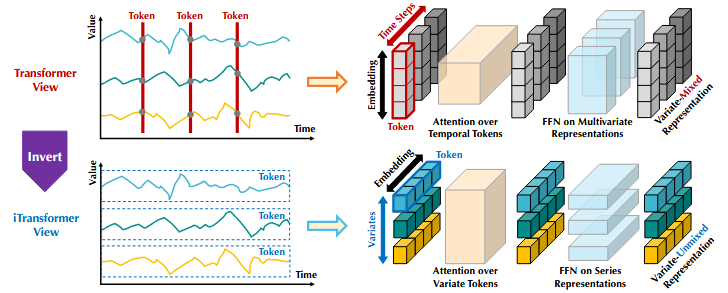
\includegraphics[width=\textwidth]{sota/iTransformer.png}
            \caption[Comparison between vanilla Transformer and iTransformer \cite{liuITransformerInvertedTransformers2023}]{Comparison between vanilla Transformer and iTransformer \cite{liuITransformerInvertedTransformers2023}}
            \label{fig::iTransformer}
 \end{figure}



\end{document}


